\section{Debugging}\label{sec:debugging}

This chapter describes how to troubleshoot QLang programs and use the provided debugging tools effectively.

% ─────────────────────────────────────────────
\subsection{The \texttt{debug()} Function and \texttt{@} Operator}\label{sec:debug-function}

The \texttt{debug()} statement is a built-in tool that dumps the internal representation of QLang objects to the console. Every line output by this command is prefixed with \texttt{DEBUG} in red text.

It operates in two distinct modes depending on whether the argument is an evaluated expression or a passed reference using the \texttt{@} operator:

\subsubsection{Expression Mode: \texttt{debug(expr)}}
When passed a standard expression, \texttt{debug()} evaluates it and prints the result's internal shape and value. For example, \texttt{debug(2 + 2)} will print the type (\texttt{Num}), shape, and the evaluated value (\texttt{4}). 

For quantum states (\texttt{state} variables), \texttt{debug(qubit)} provides a deep inspection, revealing:
\begin{itemize}
    \item \textbf{State UID:} The unique identifier of the state object.
    \item \textbf{Quantum History:} A chronological list of all gates and operations applied to that specific state.
    \item \textbf{Stabilizers:} The current stabilizer representation.
    \item \textbf{Raw State Data:} Internal amplitudes (X, Z, and Phase arrays).
\end{itemize}

\subsubsection{Reference Mode: \texttt{debug(@identifier)}}
Using the \texttt{@} prefix operator passes an entity \emph{by reference} without evaluating it. This allows you to inspect the interpreter's metadata for variables and functions.

\begin{itemize}
    \item \textbf{Variable Reference (\texttt{debug(@x)}):} Prints the symbol table metadata, including the variable's \texttt{Name}, declared \texttt{Type}, \texttt{Dimensions}, whether it \texttt{Is List}, its memory \texttt{Index}, and a recursive dump of its stored \texttt{Data}.
    \item \textbf{Function Reference (\texttt{debug(@myFunc)}):} Prints the function signature, including \texttt{Name}, \texttt{Parameter Count}, detailed parameter info (names, types, sizes, and default values), \texttt{Body Length} (number of statements), and the parsed \texttt{Position} in the source file.
\end{itemize}

% ─────────────────────────────────────────────
\Needspace{8\baselineskip}
\subsection{Example}\label{sec:debugging-example}

% Auto-generated by docs/tools/highlight.py - do not edit
\begin{codebox}
(*@\textcolor{codebox_type}{\textbf{place}}@*) (*@\textcolor{black}{my\_place}@*) (*@\textcolor{codebox_comment}{\{}@*)

    (*@\textcolor{codebox_type}{\textbf{num}}@*) (*@\textcolor{black}{my\_num}@*) (*@\textcolor{codebox_operator}{=}@*) (*@\textcolor{codebox_number}{3}@*)(*@\textcolor{codebox_operator}{;}@*)

    (*@\textcolor{codebox_type}{\textbf{num}}@*) (*@\textcolor{black}{my\_arr}@*)(*@\textcolor{codebox_operator}{[}@*)?(*@\textcolor{codebox_operator}{]}@*) (*@\textcolor{codebox_operator}{=}@*) (*@\textcolor{codebox_operator}{[}@*)(*@\textcolor{codebox_number}{42}@*)(*@\textcolor{codebox_operator}{,}@*) (*@\textcolor{codebox_number}{2.31}@*)(*@\textcolor{codebox_operator}{,}@*) (*@\textcolor{codebox_number}{32}@*)(*@\textcolor{codebox_operator}{]}@*)(*@\textcolor{codebox_operator}{;}@*)

    (*@\textcolor{codebox_type}{\textbf{text}}@*) (*@\textcolor{black}{my\_text}@*) (*@\textcolor{codebox_operator}{=}@*) (*@\textcolor{codebox_string}{\string"test\string"}@*)(*@\textcolor{codebox_operator}{;}@*)

    (*@\textcolor{codebox_type}{\textbf{state}}@*) (*@\textcolor{black}{my\_state}@*)(*@\textcolor{codebox_operator}{;}@*)

    

    (*@\textcolor{codebox_number}{debug}@*)(*@\textcolor{codebox_operator}{(}@*)(*@\textcolor{codebox_operator}{@}@*)(*@\textcolor{black}{my\_num}@*)(*@\textcolor{codebox_operator}{)}@*)(*@\textcolor{codebox_operator}{;}@*)

    (*@\textcolor{codebox_number}{debug}@*)(*@\textcolor{codebox_operator}{(}@*)(*@\textcolor{codebox_operator}{@}@*)(*@\textcolor{black}{my\_arr}@*)(*@\textcolor{codebox_operator}{)}@*)(*@\textcolor{codebox_operator}{;}@*)

    (*@\textcolor{codebox_number}{debug}@*)(*@\textcolor{codebox_operator}{(}@*)(*@\textcolor{codebox_operator}{@}@*)(*@\textcolor{black}{my\_text}@*)(*@\textcolor{codebox_operator}{)}@*)(*@\textcolor{codebox_operator}{;}@*)

    (*@\textcolor{codebox_number}{debug}@*)(*@\textcolor{codebox_operator}{(}@*)(*@\textcolor{codebox_number}{2}@*)(*@\textcolor{codebox_operator}{+}@*)(*@\textcolor{codebox_number}{2}@*)(*@\textcolor{codebox_operator}{*}@*)(*@\textcolor{codebox_number}{2}@*)(*@\textcolor{codebox_operator}{)}@*)(*@\textcolor{codebox_operator}{;}@*)

    (*@\textcolor{codebox_number}{debug}@*)(*@\textcolor{codebox_operator}{(}@*)(*@\textcolor{codebox_operator}{@}@*)(*@\textcolor{black}{my\_state}@*)(*@\textcolor{codebox_operator}{)}@*)(*@\textcolor{codebox_operator}{;}@*)

(*@\textcolor{codebox_comment}{\}}@*)




\end{codebox}


\begin{figure}[htpb]
    \centering
    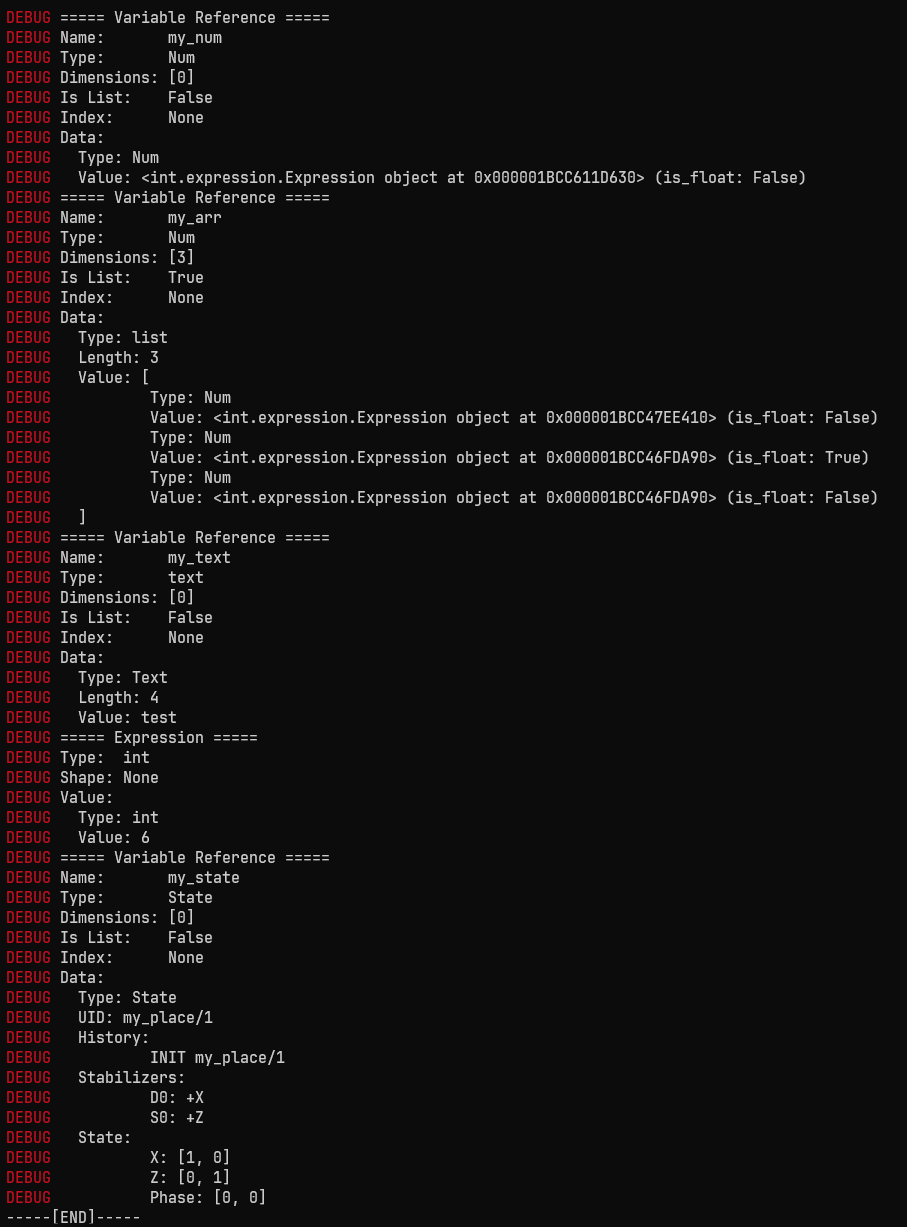
\includegraphics[width=0.9\textwidth]{img/debug_output.png}
    \caption{Output of the debugging example.}
    \label{fig:debug_demo_output}
\end{figure}

% ─────────────────────────────────────────────
\Needspace{8\baselineskip}
\subsection{Packet Logging}\label{sec:packet-logging-practice}

When building multi-place programs, a common debugging challenge is identifying deadlocks where a 
place is stuck in an infinite \texttt{receive} block, waiting for a packet that was never sent 
(or was sent with the wrong target/name). 

The \texttt{packet\_log} built-in system function enables or disables diagnostic logging for network 
activity in the current place. It is evaluated as a standard function call at runtime rather than a 
dedicated keyword. Calling \texttt{packet\_log(1)} turns logging on; \texttt{packet\_log(0)} turns 
it off. 

When enabled, every \texttt{send} and \texttt{receive} operation in that place prints detailed 
information to the interpreter's terminal, including the packet name, source, target, data size, 
and sequential packet identifier.
